\chapter{Testing and System Evaluation}
\section{System Testing}

Software testing \cite{katalon_software_testing} is the process of evaluating software to ensure it meets expected requirements. Testers run the software in controlled environments across various scenarios to identify any problems before release.

\paragraph{Why Testing Matters}

\begin{itemize}
    \item \textbf{Bug Detection}: Testing finds problems early, preventing cascading failures in interconnected systems.
    \item \textbf{Quality Assurance}: Testing ensures software remains stable, secure, and user-friendly while highlighting areas for improvement.
    \item \textbf{User Trust}: Reliable, well-tested products create positive user experiences and build customer confidence.
    \item \textbf{Risk Management}: In critical industries like healthcare and finance, testing prevents potentially harmful errors and protects against legal exposure.
\end{itemize}

\paragraph{Main Testing Categories}

Software testing falls into two primary categories:

\begin{itemize}
    \item \textbf{Functional Testing}: Verifies that features work correctly as specified
    \item \textbf{Non-functional Testing}: Examines qualities like performance, security, and usability
\end{itemize}

\paragraph{Common Testing Approaches}

The testing landscape includes many specialized methods:

\begin{itemize}
    \item \textbf{Unit Testing}: Examines individual components in isolation
    \item \textbf{Integration Testing}: Checks how components work together
    \item \textbf{End-to-End Testing}: Validates complete workflows
    \item \textbf{System Testing}: Evaluates the entire system's functionality
    \item \textbf{Exploratory Testing}: Involves freestyle investigation to discover unexpected issues
    \item \textbf{Visual Testing}: Confirms visual elements appear correctly
    \item \textbf{Regression Testing}: Ensures new code doesn't break existing features
    \item \textbf{UI Testing}: Checks user interface elements and interactions
    \item \textbf{Black-Box Testing}: Tests without knowledge of internal code
    \item \textbf{White-Box Testing}: Tests with full knowledge of code structure
    \item \textbf{Cross-Browser Testing}: Verifies compatibility across different browsers
    \item \textbf{Acceptance Testing}: Validates against real-world scenarios
    \item \textbf{Performance Testing}: Measures behavior under stress conditions
\end{itemize}
\subsection{API Testing}
For our backend application development, we implemented Postman \cite{postman_api_testing} as our solution for API storage, synchronization among team members, and manual testing procedures.
\begin{figure}[H]
    \centering
    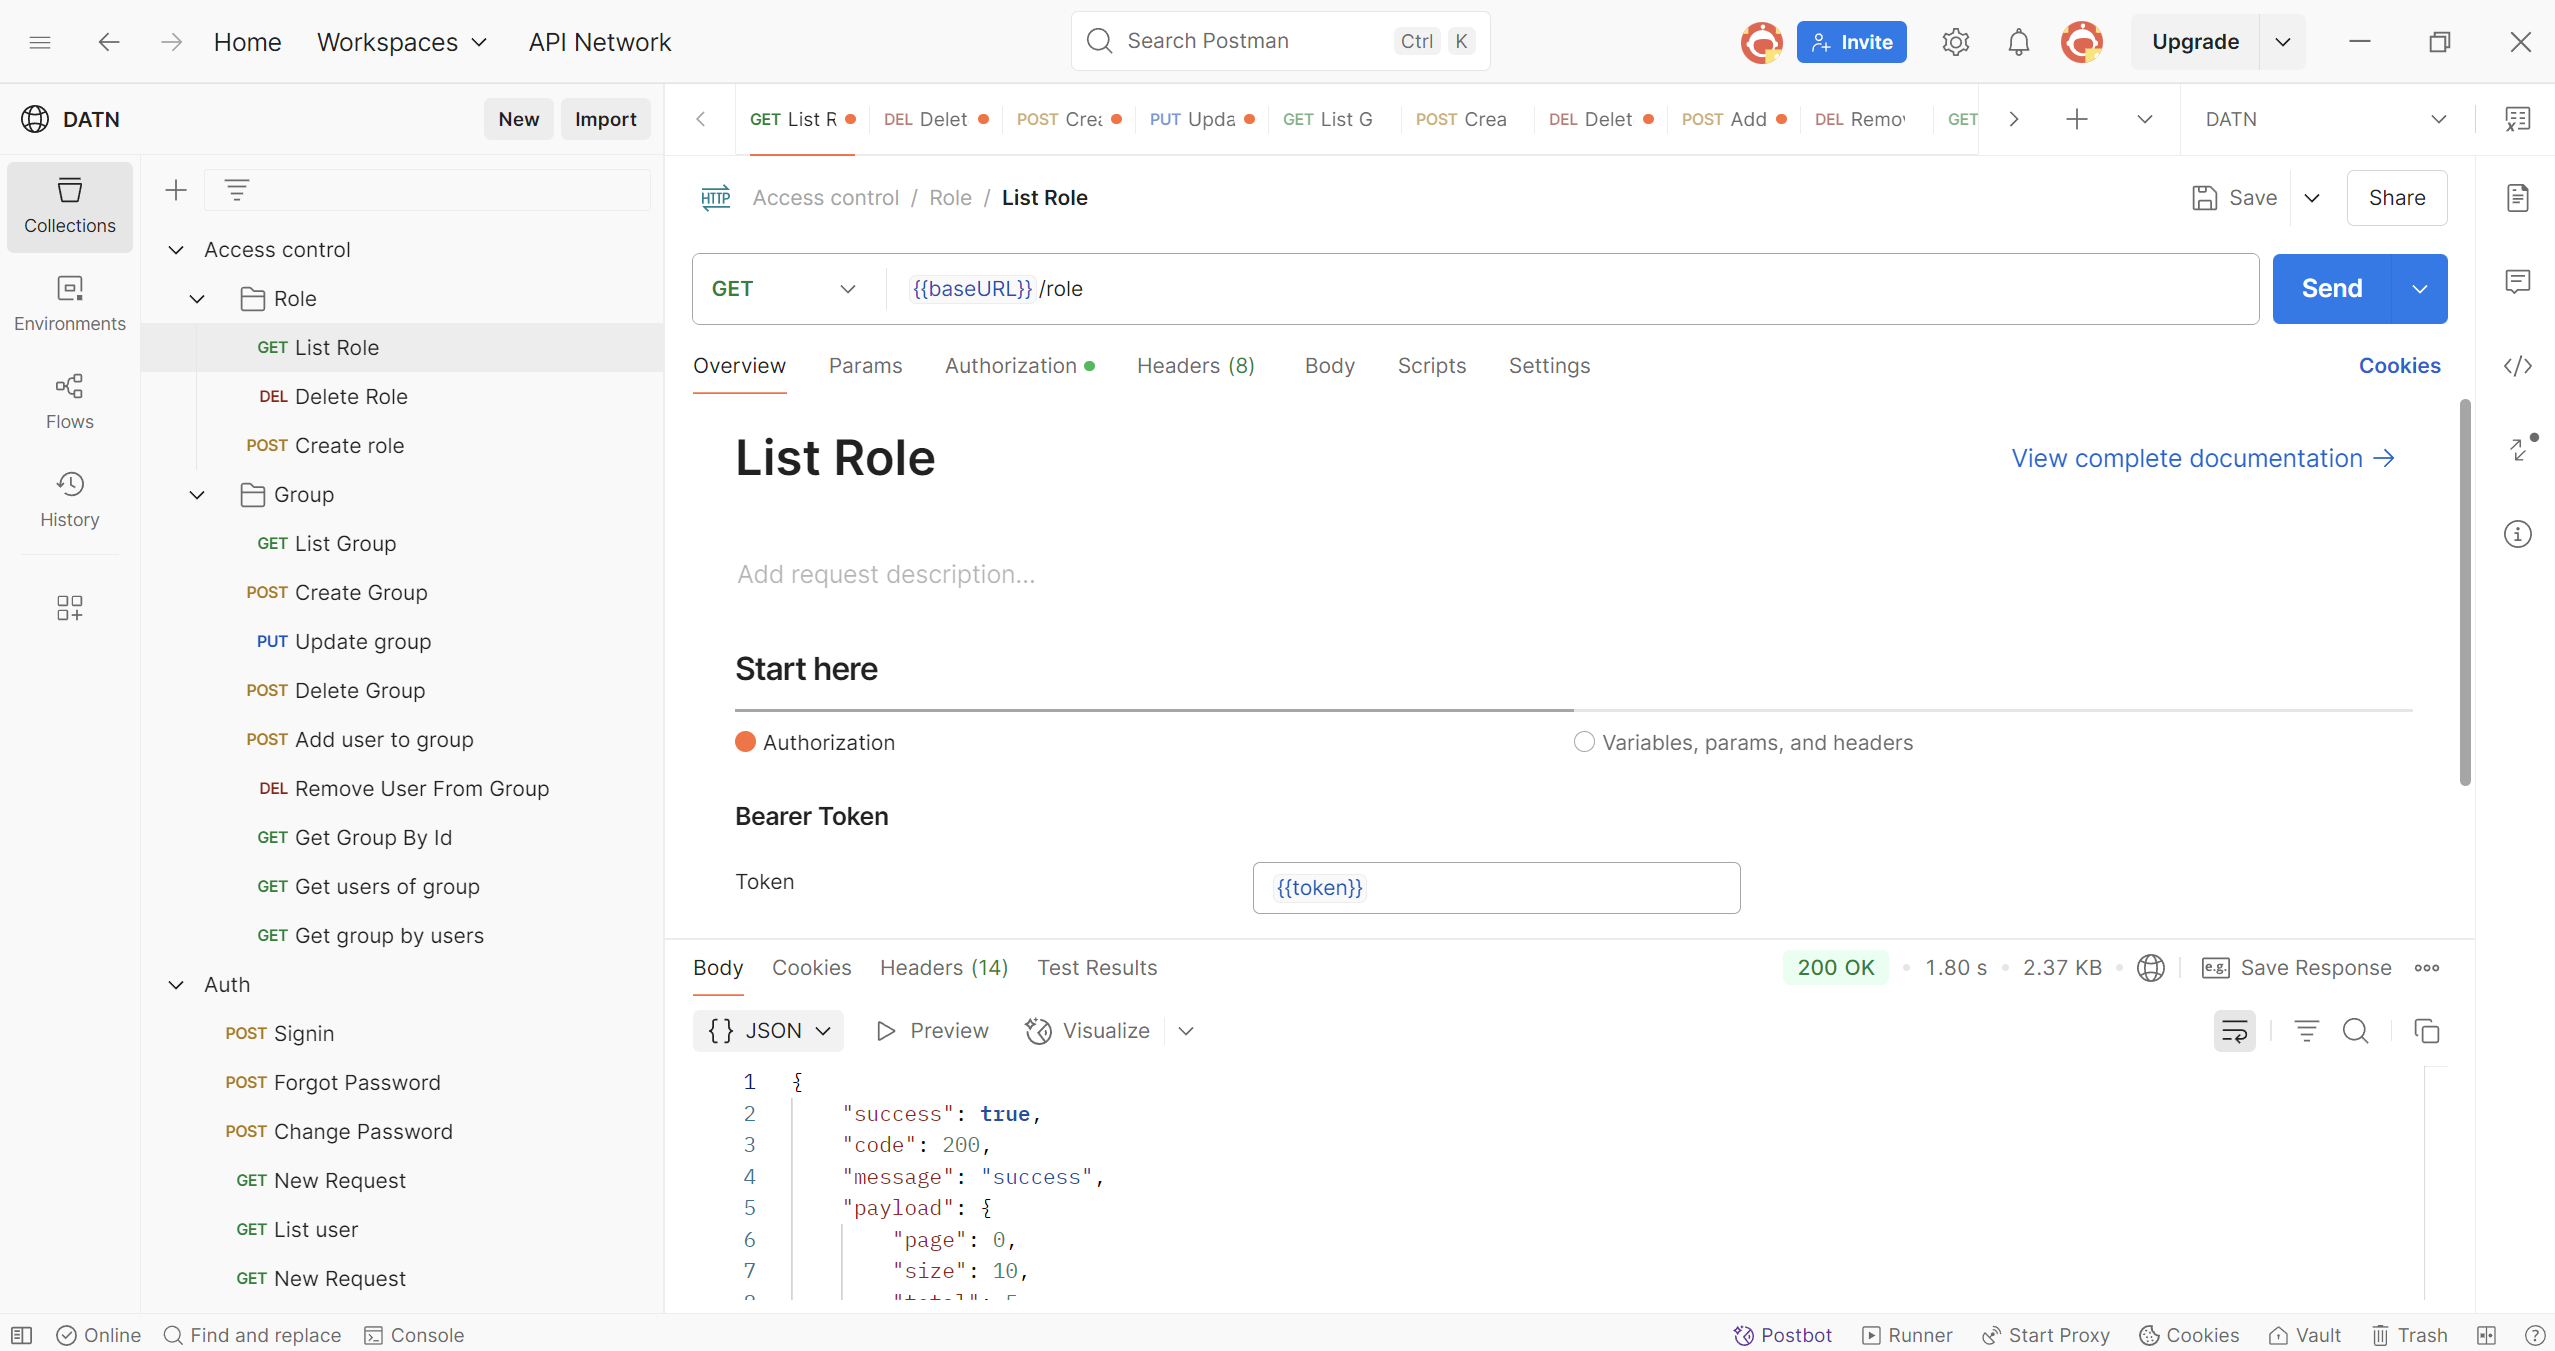
\includegraphics[width=15cm]{graphics/chapter6/postmain.png}
    \caption{API Testing with Postman}
    \label{fig:postman}
\end{figure}
\subsection{Web Interface Testing}
\subsubsection{Testing Technology Selection}
For our web interface testing, we selected Katalon Studio \cite{katalon_software_testing_intro} as our primary testing tool. This decision was based on its professional capabilities while remaining accessible for team members with limited testing experience.
\begin{figure}[H]
  \centering
  
\includegraphics[width=15cm]{graphics/chapter6/katalon.png}
  \caption{Katalon Studio}
  \label{fig:katalon}
\end{figure}

Katalon Studio is a comprehensive automation testing solution for web and mobile applications. It provides a complete package of powerful features designed to overcome common challenges in web interface automation testing, such as handling pop-ups, iFrames, and wait-time issues.

This user-friendly and flexible solution enhances testing efficiency, allowing testers to work faster and deploy higher quality software through intelligent automation support throughout the testing process. The implementation of this tool was particularly valuable for our customer portal system development in the transportation and logistics sector.

\subsubsection{Key Features of Katalon Studio}

\begin{itemize}
    \item \textbf{Rapid Test Case Development}: Supports both Manual and Scripting modes for efficient test creation
    \item \textbf{Multi-Platform Testing Capabilities}: Enables testing of Web applications, APIs, mobile and desktop applications
    \item \textbf{Cross-Platform Compatibility}: Functions across Windows, Linux, and macOS operating systems
    \item \textbf{Codeless Testing Support}: Offers Spy and Record functionalities to create test cases without coding requirements
    \item \textbf{Data-Driven Testing}: Compatible with external data sources including Excel, CSV files, and database connections
    \item \textbf{BDD Testing Support}: Facilitates Behavior-Driven Development testing approaches
    \item \textbf{Integration Capabilities}: Supports command line execution, CI/CD integration, and expandable functionality through plugins
    \item \textbf{Pre-built Testing Components}: Includes built-in keywords for web, API, mobile, and desktop application testing
\end{itemize}

\subsubsection{Testing Process}
\begin{itemize}
  \item \textbf{Plan}: Use features Web Recorder and Spy to create test cases and test suites
  \item \textbf{Download and Install Katalon Studio}: 
  \begin{enumerate}
    \item Visit the Katalon Studio website and download the latest version of Katalon Studio.
    \item Run the installation file and follow the on-screen instructions to complete the setup process.
    \item Launch Katalon Studio and create a free account or log in with existing credentials.
    \item After installation, we will get the following interface: \begin{figure}[H]
      \centering
      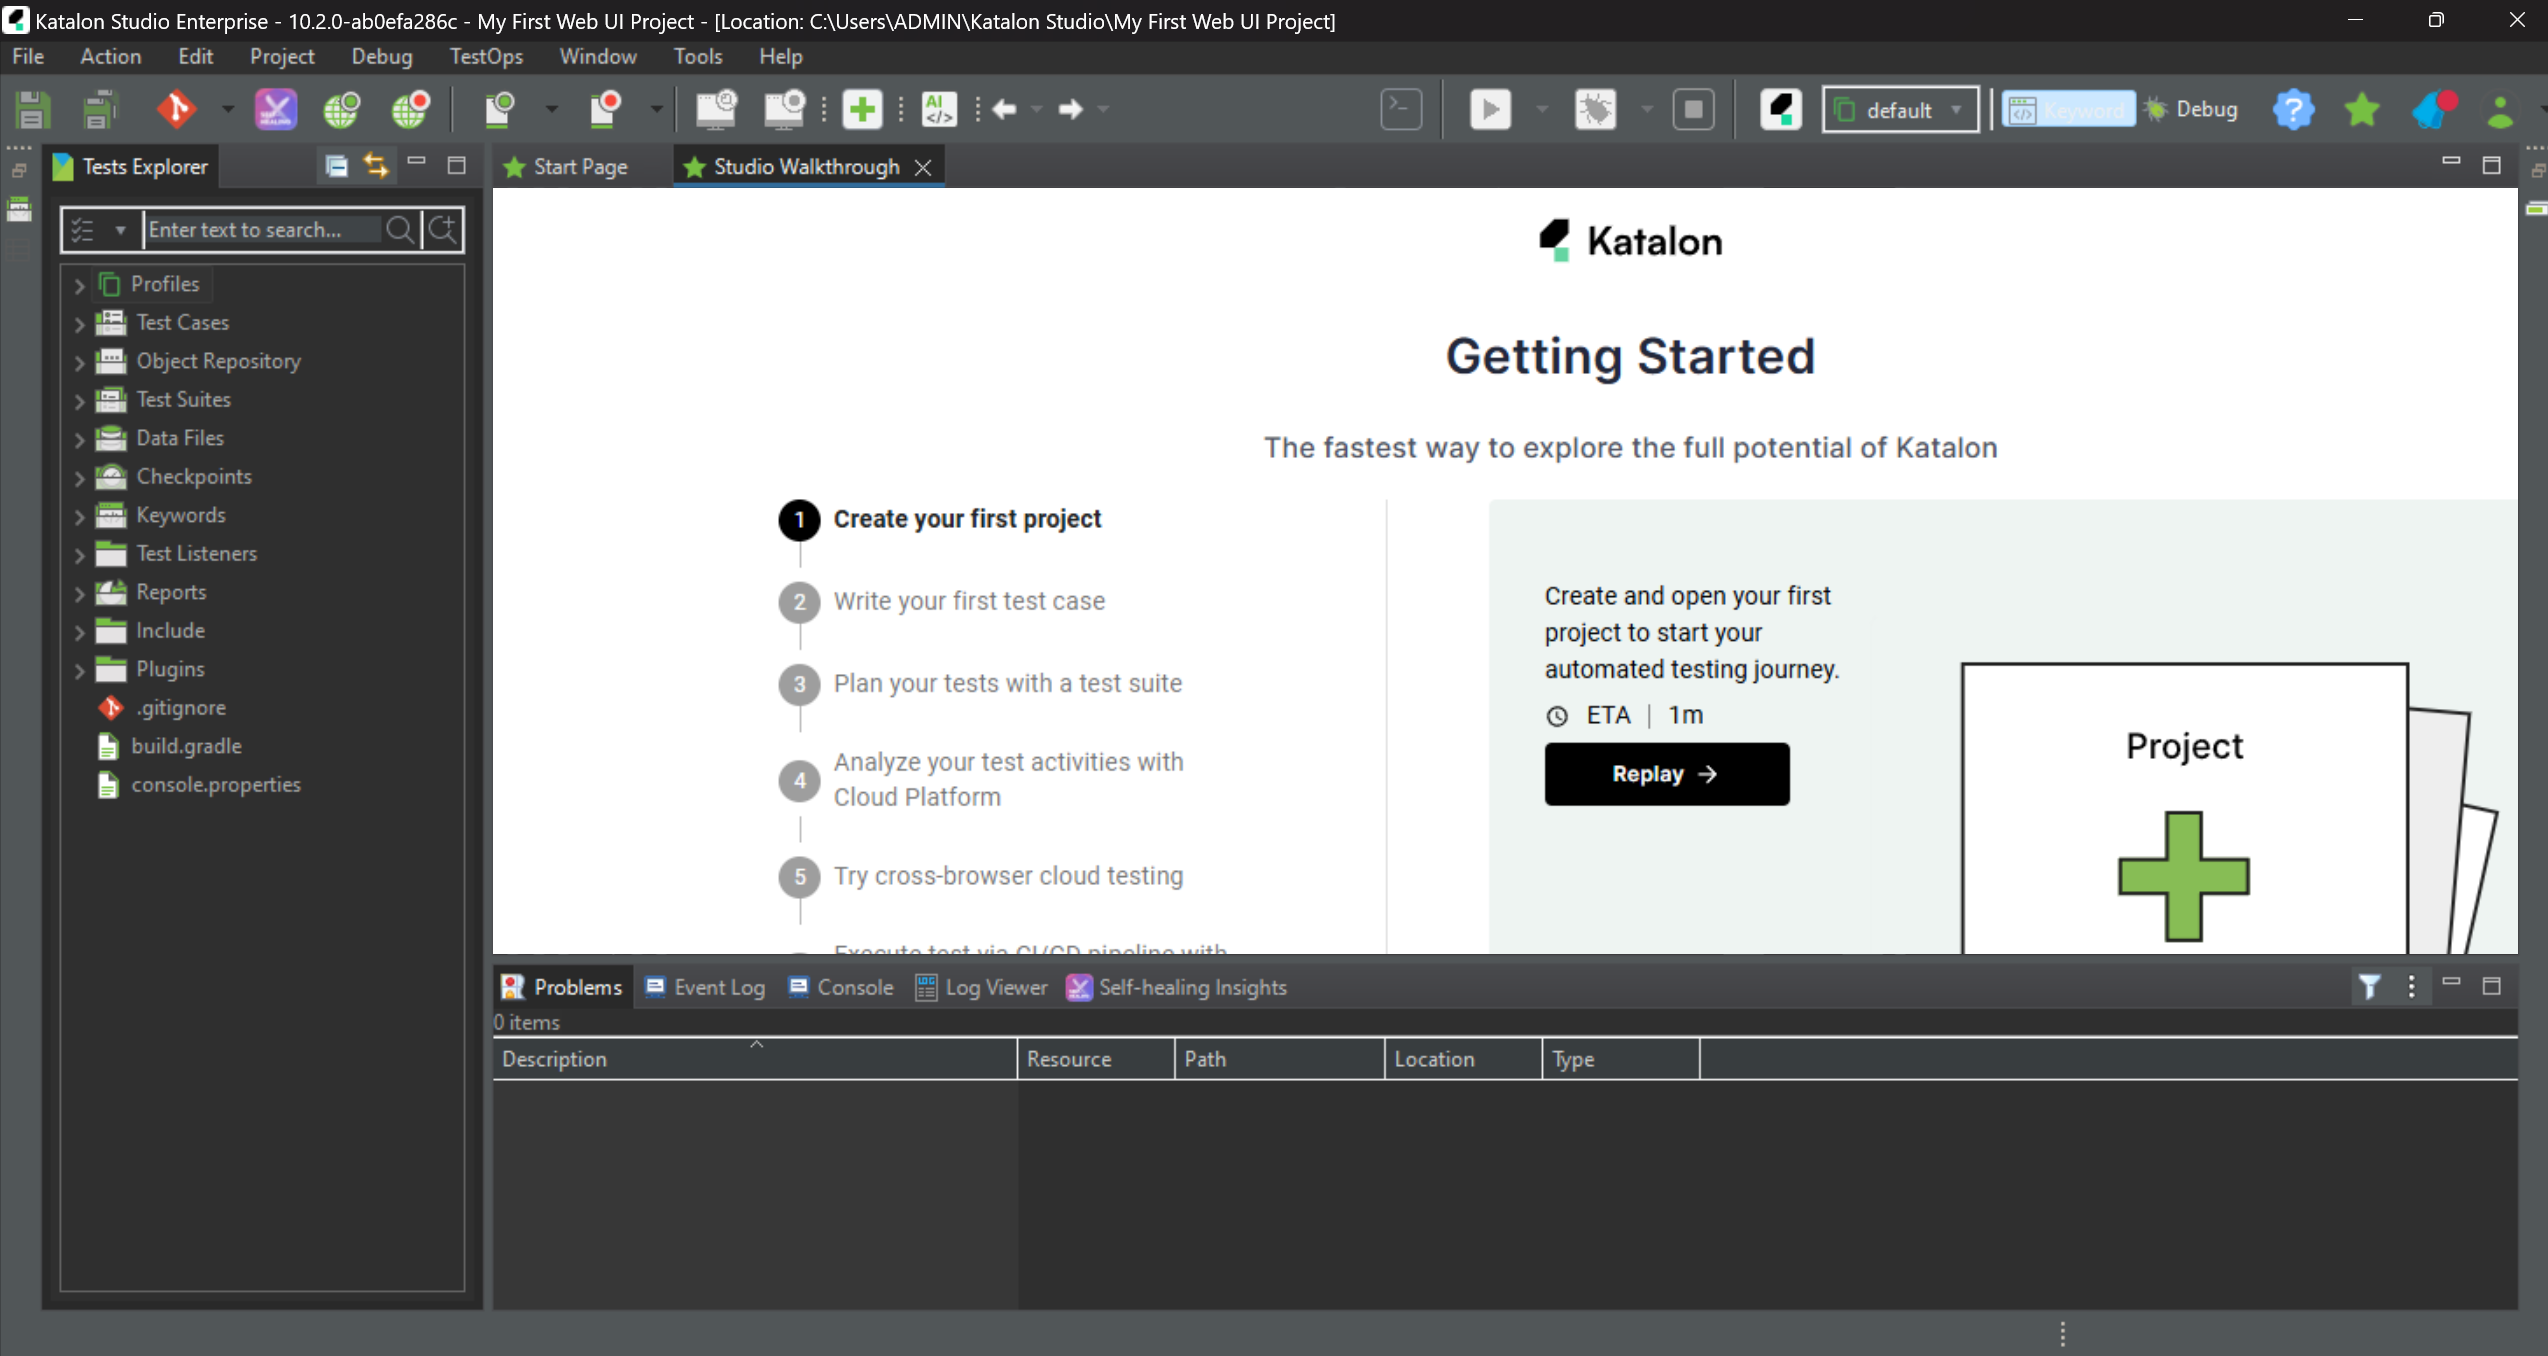
\includegraphics[width=15cm]{graphics/chapter6/katalon_installation.png}
      \caption{Katalon Studio Installation}
      \label{fig:katalon_installation}
    \end{figure}
  \end{enumerate}
  \item \textbf{Create a New Project for Testing}
  \item \textbf{Create Test suites}: Create test suites to group related test cases for efficient execution
  \begin{figure}[H]
    \centering
    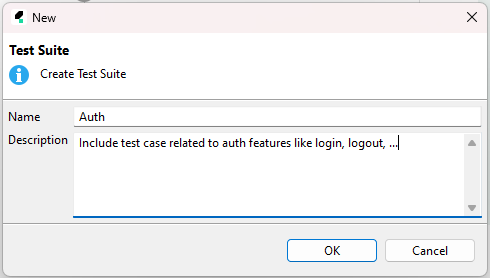
\includegraphics[width=0.5\textwidth]{graphics/chapter6/new_test_suite.png}
    \caption{Create Test Suite}
    \label{fig:newtest_suite}
  \end{figure}
  \item \textbf{Add Test Cases to Test Suites}: Add test cases to the test suite created in the previous step. We will use Web Recorder to create test cases.
  \begin{figure}[H]
    \centering
    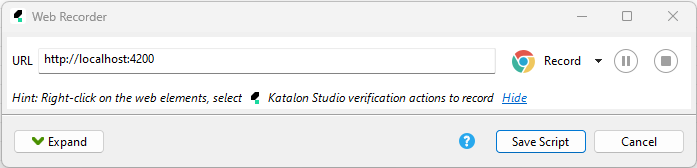
\includegraphics[width=0.5\textwidth]{graphics/chapter6/web_recorder.png}
    \caption{Web Recorder}
    \label{fig:web_recorder}
  \end{figure}
  \item \textbf{Run Test Suites}: Execute the test suites to validate the functionality of the web application. Katalon Studio will automatically run the test cases in the specified order and generate a report with the results.
\end{itemize}
\subsubsection{Testing Results}
\begin{itemize}
  \item \textbf{Test Suite Auth}: Login and logout functionality
  \begin{table}[H]
    \centering
    \caption{Authentication Test Cases}
    \begin{tabular}{|p{4cm}|p{5cm}|p{4cm}|p{1cm}|}
    \hline
    \textbf{Test Case} & \textbf{Description} & \textbf{Expected Result} & \textbf{Result} \\
    \hline
    Login with valid credentials & User enters correct username and password & User is authenticated and redirected to dashboard & Pass \\
    \hline
    Login with invalid credentials & User enters incorrect username or password & System displays error message and prevents access & Pass \\
    \hline
    User Logout &   User clicks logout button & User is logged out and redirected to login page & Pass \\
    \hline
    Login with admin credentials & Users enter admin username and password & User is authenticated and redirected to admin dashboard & Pass \\
    \hline
    \end{tabular}
    \label{tab:auth_tests}
  \end{table}
  \textbf{Kalaton Studio Test Suite Auth results:} 
  \begin{figure}[H]
    \centering
    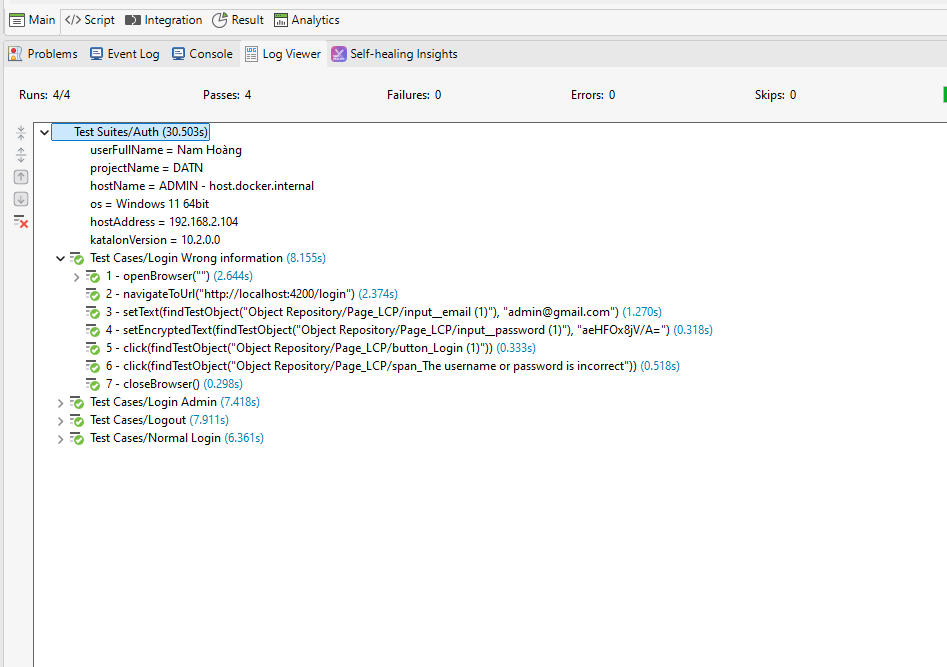
\includegraphics[width=15cm]{graphics/chapter6/test_suite_auth.png}
    \caption{Test Suite Auth Results}
    \label{fig:test_suite_auth}
  \end{figure}
  \item \textbf{Test Suite Client}: Client management functionality
  \begin{table}[H]
  \centering
  \caption{Client Management Test Cases}
  \begin{tabular}{|p{4cm}|p{5cm}|p{4cm}|p{1cm}|}
  \hline
  \textbf{Test Case} & \textbf{Description} & \textbf{Expected Result} & \textbf{Result} \\
  \hline
  View client & User navigates to client listing page & System displays list of all clients with pagination and search functionality & Pass \\
  \hline
  New client & User completes and submits the new client form with valid data & System creates new client and displays success message & Pass \\
  \hline
  Edit client & User modifies client information and saves changes & System updates client information and displays confirmation message & Pass \\
  \hline
  \end{tabular}
  \label{tab:client_tests}
  \end{table}
  \textbf{Kalaton Studio Test Suite Client results:} 
  \begin{figure}[H]
    \centering
    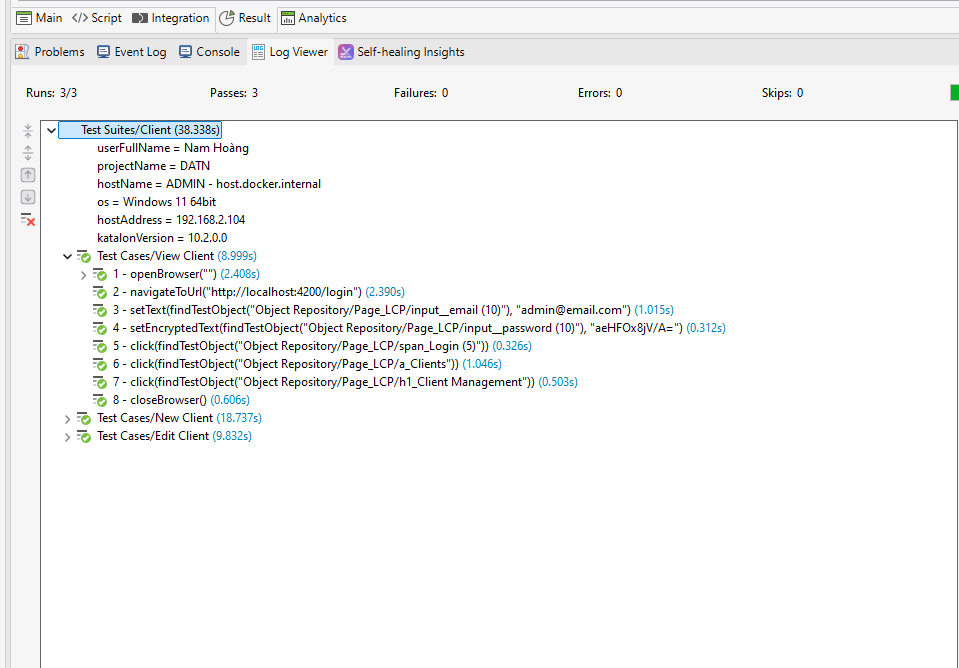
\includegraphics[width=15cm]{graphics/chapter6/test_suite_client.png}
    \caption{Test Suite Client Results}
    \label{fig:test_suite_client}
  \end{figure}
  \item \textbf{Test Suite Freight Rate Management}: Freight Rate management functionality
  \begin{table}[H]
  \centering
  \caption{Freight Rate Management Test Cases}
  \begin{tabular}{|p{4cm}|p{5cm}|p{4cm}|p{1cm}|}
  \hline
  \textbf{Test Case} & \textbf{Description} & \textbf{Expected Result} & \textbf{Result} \\
  \hline
  View freight rate & User navigates to freight rate listing page & System displays list of all freight rate with pagination and search functionality & Pass \\
  \hline
  New freight rate & User completes and submits the new freight rate form with valid data & System creates new freight rate and displays success message & Pass \\
  \hline
  Edit freight rate & User modifies freight rate information and saves changes & System updates freight rate information and displays confirmation message & Pass \\
  \hline
  \end{tabular}
  \label{tab:freight_rate_test}
  \end{table}
  \textbf{Kalaton Studio Test Suite Freight Rate Management results:} 
  \begin{figure}[H]
    \centering
    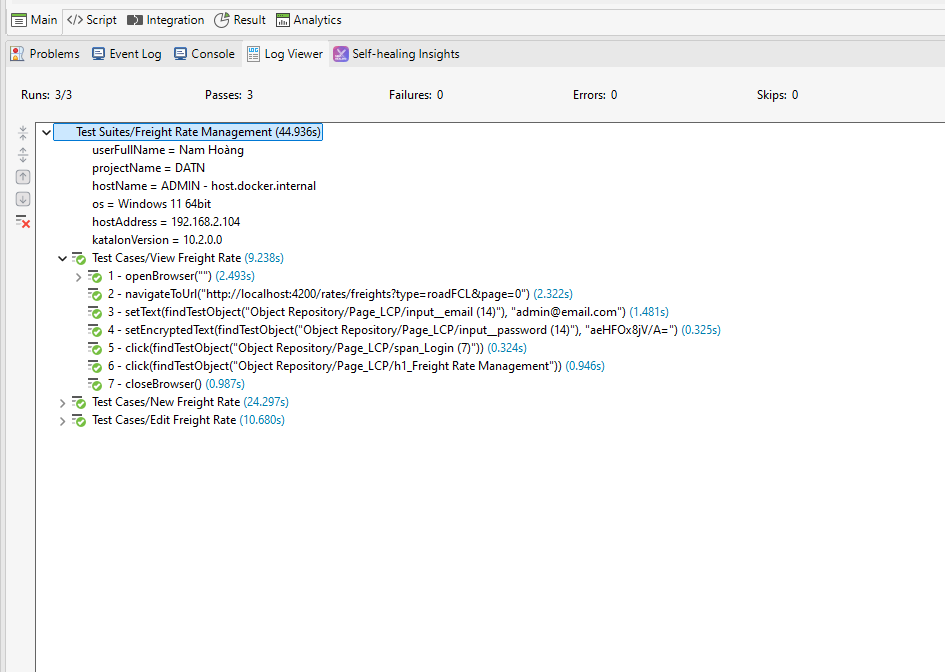
\includegraphics[width=15cm]{graphics/chapter6/test_suite_freight_rate.png}
    \caption{Test Suite Freight Rate Management Results}
    \label{fig:test_suite_freight_rate_management}
  \end{figure}
  \item \textbf{Test Suite Users Management}: Users management functionality
  \begin{table}[H]
  \centering
  \caption{Users Management Test Cases}
  \begin{tabular}{|p{4cm}|p{5cm}|p{4cm}|p{1cm}|}
  \hline
  \textbf{Test Case} & \textbf{Description} & \textbf{Expected Result} & \textbf{Result} \\
  \hline
  View Users & User navigates to User listing page & System displays list of all User with pagination and search functionality & Pass \\
  \hline
  New User & User completes and submits the new User form with valid data & System creates new User and displays success message & Pass \\
  \hline
  Search User & User search user by name & System display corresponding results & Pass \\
  \hline
  \end{tabular}
  \label{tab:users_test}
  \end{table}
  \textbf{Kalaton Studio Test Suite Users Management results:} 
  \begin{figure}[H]
    \centering
    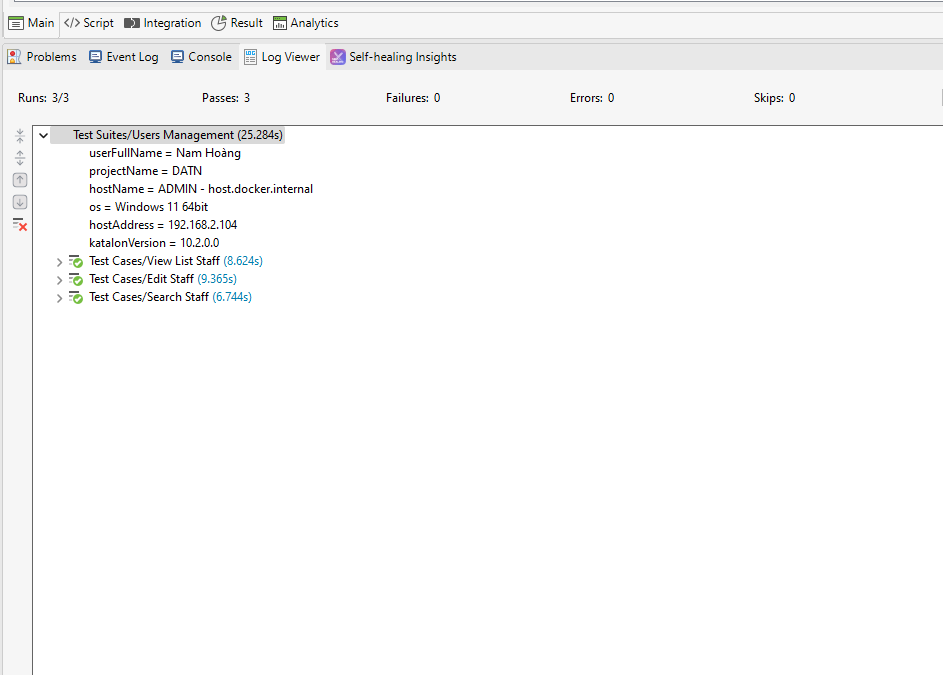
\includegraphics[width=15cm]{graphics/chapter6/test_suite_users.png}
    \caption{Test Suite Users Management Results}
    \label{fig:test_suite_users_management}
  \end{figure}
\end{itemize}

\section{System Evaluation}
Google PageSpeed Insights \cite{google_page_speed} is a suite of tools developed by Google designed to optimize web page performance. It primarily focuses on two key aspects: page loading speed and user experience. These components adhere to Google's web performance methodologies while automating the optimization process.

Google offers Lighthouse, an open-source automated tool aimed at improving website quality using the Google PageSpeed metrics. Users can apply this tool to any website, and it has the capability to access browser-stored data such as tokens. This Google Chrome Audit tool evaluates various aspects including performance, accessibility, SEO, and other parameters, providing corresponding scores.

To assess website performance using Lighthouse, users need to install the Lighthouse extension, open DevTools, select the Lighthouse tab, and choose ``Analyze page load." Lighthouse then runs a series of tests on the page and compiles the results into a comprehensive performance report. Based on these findings, users can make targeted improvements to enhance their website's overall performance.
\subsection{Evaluation results}
Using Lighthouse to evaluate the performance of our web application, we obtained the following results:
\begin{figure}[H]
  \centering
  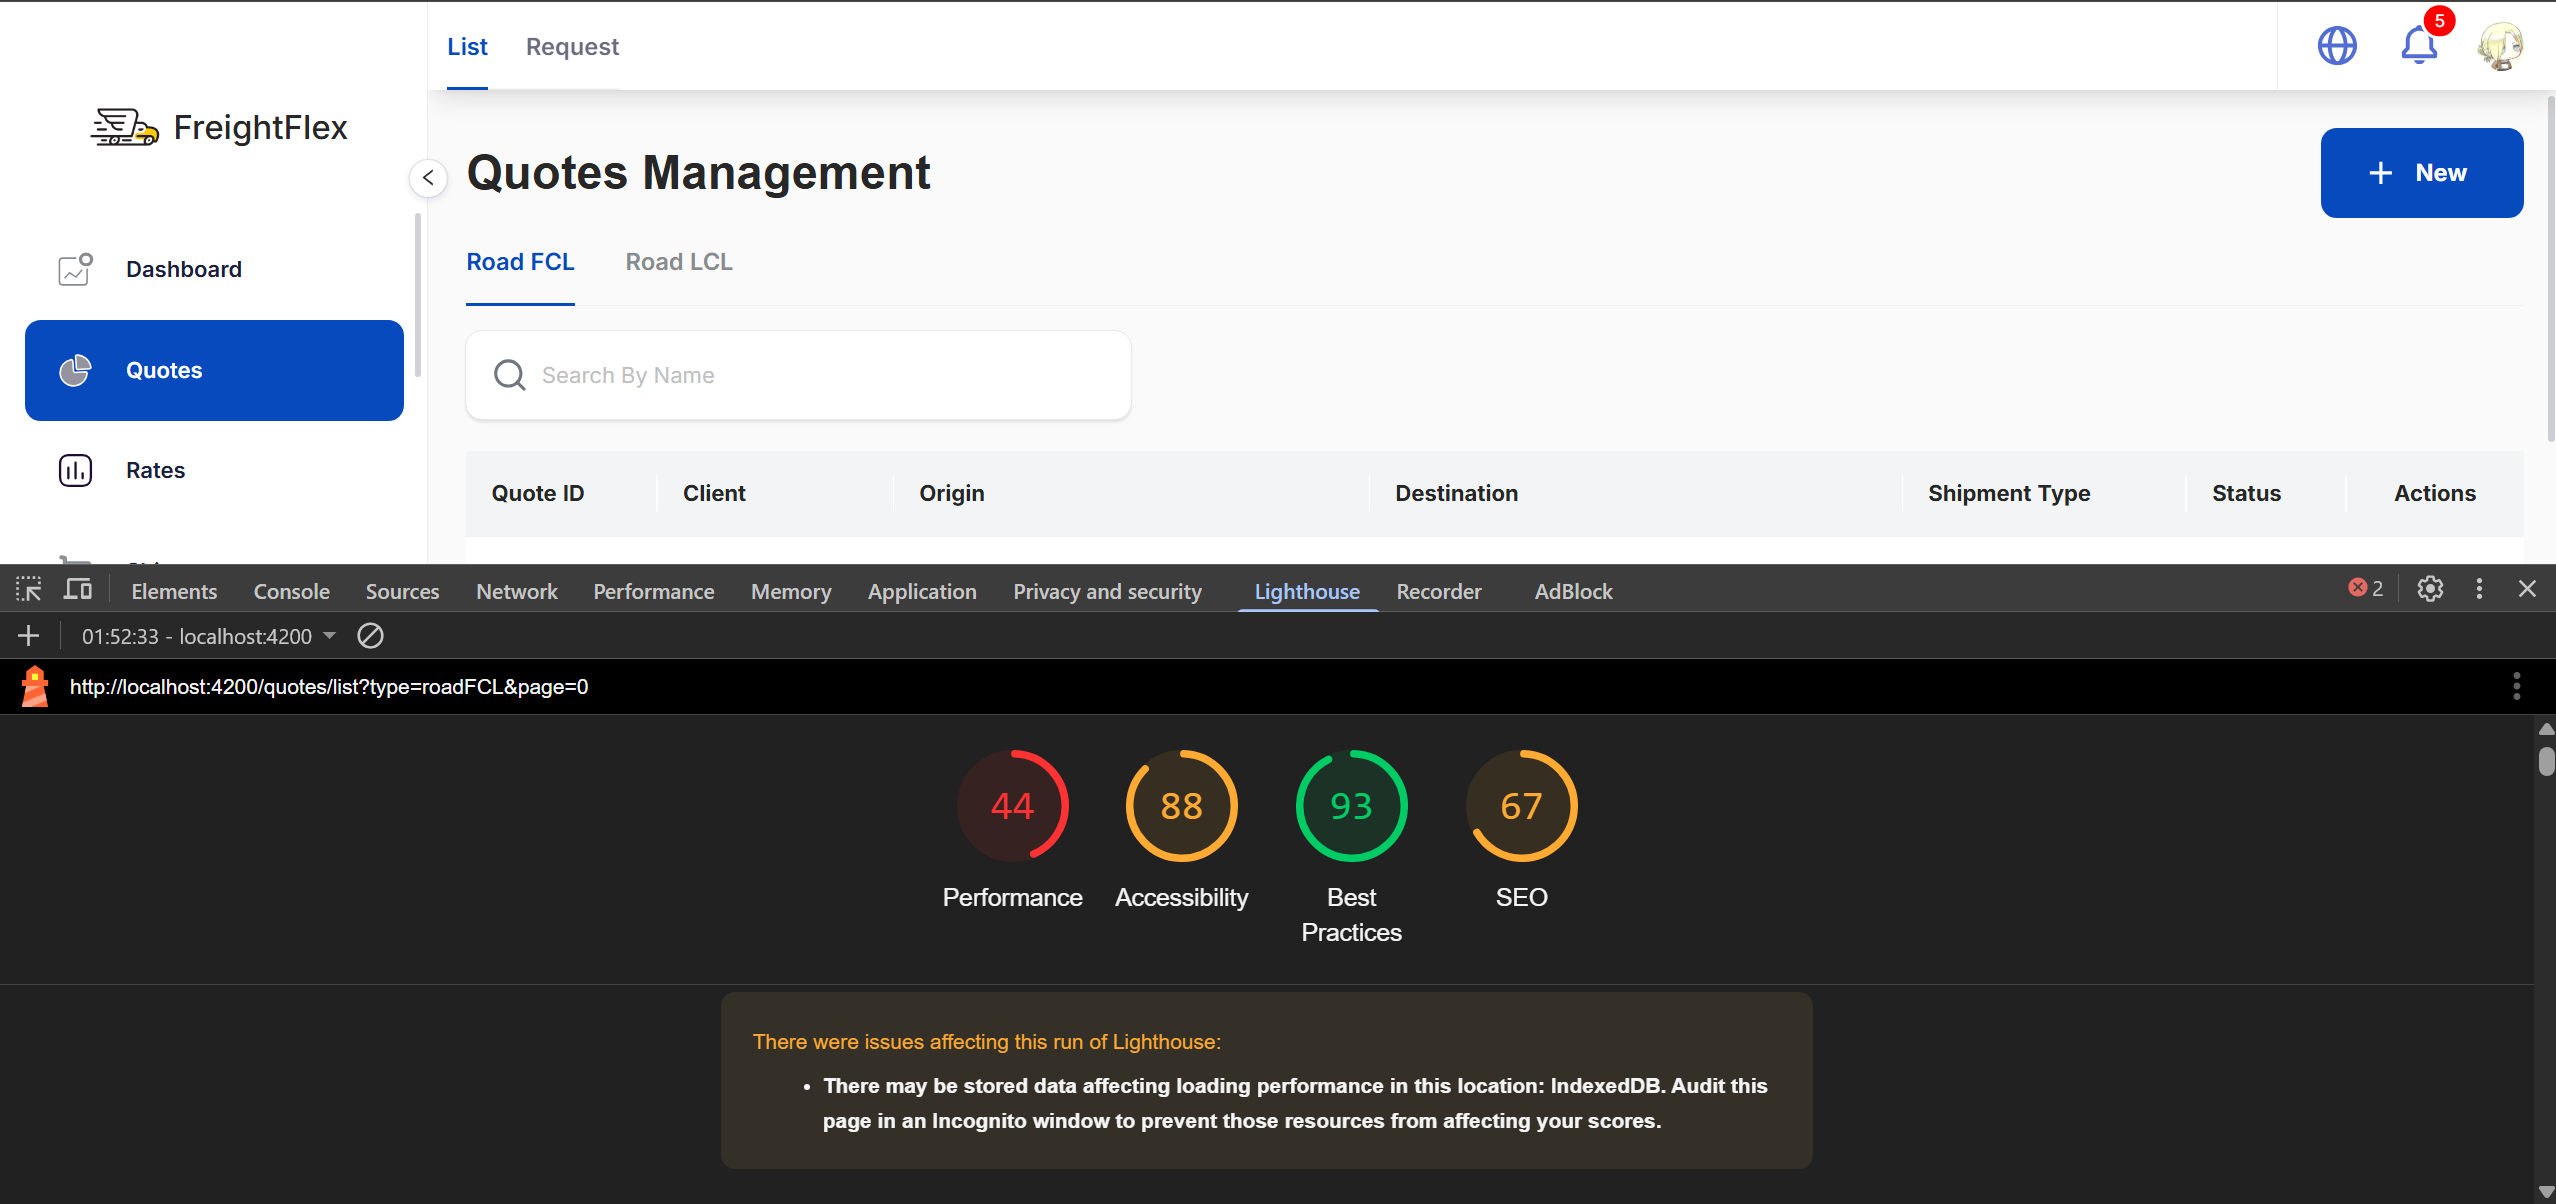
\includegraphics[width=15cm]{graphics/chapter6/quotes.png}
  \caption{Quotes page performance evaluation}
  \label{fig:quotes}
\end{figure}

\begin{figure}[H]
  \centering
  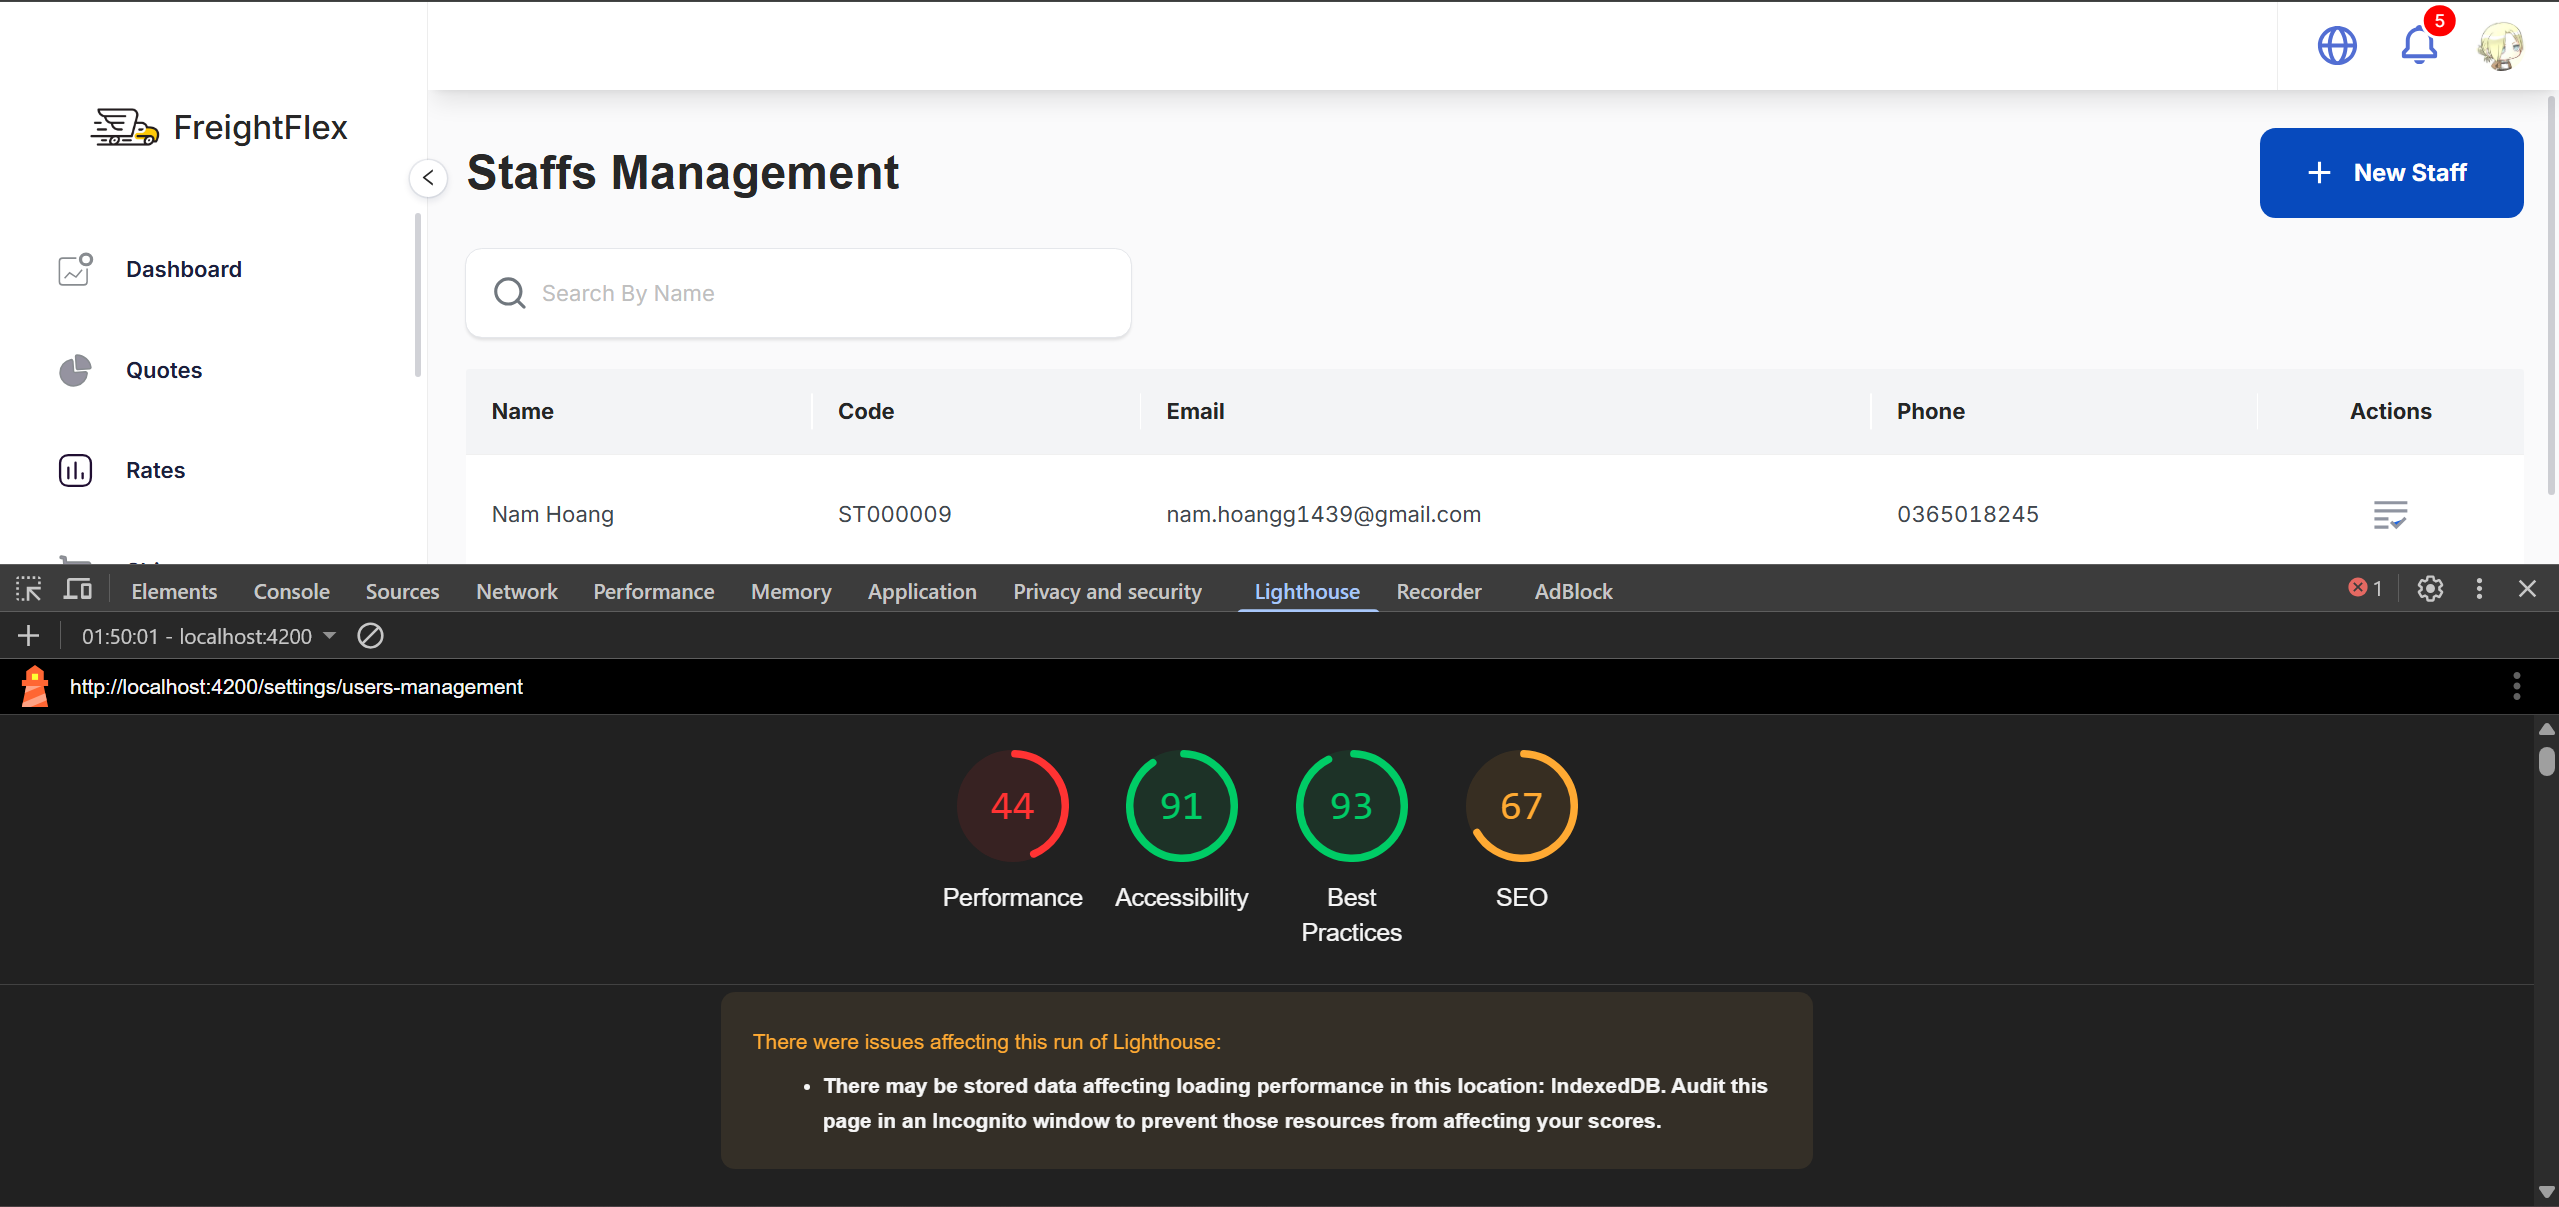
\includegraphics[width=15cm]{graphics/chapter6/staff_before.png}
  \caption{Staff page performance evaluation}
  \label{fig:staff_before}
\end{figure}

\noindent The performance evaluation revealed scores ranging between 40 and 45, which falls below the threshold considered acceptable for modern web applications. In contrast, other metrics achieved values exceeding 60, which is generally regarded as satisfactory performance.

We implemented various optimization strategies based on Lighthouse recommendations, which resulted in notable improvements in the Best Practices metric. However, despite these interventions, the performance score remained consistently low. Analysis indicates this is primarily attributable to the application's dependence on resource-intensive JavaScript libraries and complex computational logic.

Current constraints on time and resources prevent implementation of comprehensive performance optimizations. Nevertheless, a systematic optimization strategy has been developed for implementation in subsequent development phases to address these performance limitations.

